\section{Experimental and Reporting Details}\label{app:training}\label{app:conventions}

The following details supplement the model and admission rule in Section~\ref{sec:setting}.
Training uses float64 throughout. Each architecture has $20$ spatial and $20$ temporal
sub-networks of widths $[\,\cdot\,,64,64,1]$ feeding a $[40,128,128,1]$ fusion head.
Activations are $\tanh$, biases are initialised to zero and weights are drawn from
$\mathcal N(0,2/d_{\rm in})$. Fourier models use $16$ random features per axis, with
bandwidth $2$ for Burgers and $1$ for Allen--Cahn. Adam has learning rate $10^{-3}$,
with $5000$ Burgers steps and $15{,}000$ Allen--Cahn steps, followed by $50$ and $200$
Levenberg--Marquardt steps. Each LM step uses at most $100$ CG iterations, initial
damping $10^{-4}$ and minimum $10^{-12}$; it accepts at $\rho_{\rm LM}>0.25$, divides
damping by $3$ at $\rho_{\rm LM}>0.75$ and multiplies it by $4$ on rejection, allowing
at most $5$ consecutive rejections. Residual row counts and weights are given in
Section~\ref{sec:setting}; complete implementation settings are preserved with the code.

Reported multi-run means average per-run quantities. Every $\pm$ denotes the population
standard deviation with divisor $n$; ranges give observed minima and maxima.
The three-run control varies paired pulse-width/diffusivity settings at seed $0$.
Mean gaps are means of ratios, not ratios of mean contrasts: on Burgers--MLP they are
$20.47$ and $20.49$, respectively. Reference-error oracles are evaluation devices,
not training-based tuning rules.

A common $2\%$ admission cutoff retains $13/17$ of the original cohort:
$8/8$ Burgers--MLP, $3/3$ Burgers--Fourier, Allen--Cahn MLP seed $3$ and
Allen--Cahn Fourier seed $1$. The original $3\%$ Allen--Cahn cutoff remains a
convention, not a PDE-derived tolerance. The unchanged masks and saved fields
permit the subset comparison below; its two Allen--Cahn results are single-run
descriptions. In this subset, the baseline zero-mean affine error increases in
$10/13$ runs; direct $\theta$-centred baseline predictions give $\rho^\theta>1$ in
all $13$, including the one case unresolved by the $12/13$ bound.
With trained centres, conditional-MLE sharp coverage is below nominal in all $13$ runs:
$[0.018,0.62425]$ at one sigma and $[0.051,0.768]$ at $1.96$ sigma. Bulk
coverage is below nominal in $10/13$ and $12/13$ runs at those thresholds,
respectively. All eight Burgers--MLP findings and the five refined trained-centre
crossings remain in this subset by construction.

\emph{Linear-control context.}
The contextual linear control solves $u_t+a u_x=\nu u_{xx}$ with $a=1$ and a
periodic Gaussian pulse. Three of four MLP attempts pass admission; the admitted
seed-$0$ runs vary paired pulse-width/diffusivity settings. At the baseline their
uncertainty contrasts are $[1.086,1.331]$, error contrasts $[0.7816,0.9986]$ and
gaps $[0.6521,0.899]$. They are not part of the nonlinear $17$-run scale study.

\emph{Grid and spectral checks.}\label{app:grid}\label{app:spectralchecks}
The top-$5\%$ region rule alone does not establish feature resolution. For the sharpest
slice, the discrete integral width in cells is
\[
 W_{\rm cells}=\frac{\sum_j|\partial_xu^\ast(x_j,t)|}{\max_j|\partial_xu^\ast(x_j,t)|}.
\]
This effective discrete width avoids the crossing-count floor of the half-maximum
statistic; exceeding one cell does not establish continuum resolution. On nested
spatial subsamples with recomputed masks, primary RMS and secondary mean-width
contrasts change by at most $1.1\%$ between $n_x=400$ and $200$. This sampling-density
check concerns baseline contrasts, not convergence of oracle coverage. The canonical Gram spectral projectors were checked for
orthonormality, separation at the cutoff and eigenpair backward error; independent
Woodbury evaluations checked variances. The all-17 direct-$J$ checks are summarised
in Appendix~\ref{app:r2:numerics}, with numerical protocols in Appendix~\ref{oa:numerics}.

\section{Spectral Bounds and Aggregation}\label{app:aggregation}

We give the proofs supporting the two-subspace summaries
in Section~\ref{sec:theory} and their aggregation to regional statistics.

\begin{theorem}[Two-sided spectral sandwich]\label{thm:ceiling}
For $F\succeq0$, $\alpha,\epsilon>0$ and $g_\bk\ne0$,
\begin{equation}\label{eq:sandwich}
 L(\epsilon):=\frac{m_\epsilon(g_\sh)}{M_\epsilon(g_\bk)}
 \le\frac{\sigma^2(g_\sh)}{\sigma^2(g_\bk)}
 \le\frac{M_\epsilon(g_\sh)}{m_\epsilon(g_\bk)}=:U(\epsilon).
\end{equation}
Consequently, the ratio lies between $\sup_{\epsilon>0}L(\epsilon)$ and
$\inf_{\epsilon>0}U(\epsilon)$.
\end{theorem}
\begin{proof}
In the weak block, $\alpha\le\alpha+\lambda_i\le\alpha+\epsilon$; in the strong
block, $\alpha+\epsilon<\alpha+\lambda_i\le\alpha+\lambda_{\max}$.
Applying reciprocal bounds to \eqref{eq:sigma-sum} gives
$m_\epsilon(g)\le\sigma^2(g)\le M_\epsilon(g)$.
Both bulk envelopes are positive, so division in opposite directions gives the result.
\end{proof}

The primary statistic averages variance before taking square roots. The secondary
mean-width ratio is $\achratio=\langle\sigma(g)\rangle_{\mathcal S}/
\langle\sigma(g)\rangle_{\mathcal B}$. Uniform pairwise bounds also transfer to it:
if $\ell\sigma(g_b)\le\sigma(g_s)\le u\sigma(g_b)$ for every sharp--bulk pair, averaging
over both finite regions and dividing by positive bulk mean width gives
$\ell\le\achratio\le u$. This differs from evaluating variance at a region-mean tangent.

For regions with positive mean width, define
$\kappa_r=\sigma(\langle g\rangle_r)/\langle\sigma(g)\rangle_r$.
The covariance norm triangle inequality gives $0\le\kappa_r\le1$, and cancellation
of the two mean widths gives, when $\kappa_{\mathcal B}>0$,
\begin{equation}\label{eq:ratio-identity}
 \frac{\sigma(\langle g\rangle_{\mathcal S})}{\sigma(\langle g\rangle_{\mathcal B})}
 =\frac{\kappa_{\mathcal S}}{\kappa_{\mathcal B}}\achratio.
\end{equation}
Equation~\eqref{eq:ratio-identity} shows why mean-tangent loadings cannot replace
the primary pointwise energies. The following sharpness result concerns the
information in those energies.

\emph{Sharpness of the spectral bounds.}\label{app:sharpness}
The following construction shows what can be inferred from the four block energies alone.
It does not assert that measured networks attain the bounding envelopes.

\begin{proposition}[Sharpness]\label{prop:sharp}
Fix $\alpha>0$, $0<\epsilon<\lambda_{\max}$ and four nonnegative block energies,
with positive total bulk energy. Spectra and vectors realising these energies can
approach either endpoint of \eqref{eq:sandwich}.
\end{proposition}
\begin{proof}
For $\epsilon<\epsilon'\le\lambda_{\max}$, use four orthogonal modes with eigenvalues
$0,\epsilon,\epsilon',\lambda_{\max}$. To approach $U$, place the sharp weak and
strong energies at $0,\epsilon'$, and the bulk energies at $\epsilon,\lambda_{\max}$.
Square-root coordinates realise the prescribed energies and give
\[
 \frac{q_{\sh,\rm sl}/\alpha+q_{\sh,\rm st}/(\alpha+\epsilon')}
      {q_{\bk,\rm sl}/(\alpha+\epsilon)+q_{\bk,\rm st}/(\alpha+\lambda_{\max})}
 \longrightarrow U(\epsilon)\quad(\epsilon'\downarrow\epsilon).
\]
For $L$, place sharp energies at $\epsilon,\lambda_{\max}$ and bulk energies at
$0,\epsilon'$. The ratio then tends to $L(\epsilon)$. The strict inequality
$\epsilon'>\epsilon$ keeps that mode in the strong block.
\end{proof}


\section{Full-Grid Scale and Centre Diagnostics}\label{app:r2}

These diagnostics use all $17$ admitted checkpoints: Burgers--MLP seeds $0$--$7$,
Burgers--Fourier seeds $0,2,6$, and Allen--Cahn MLP/Fourier seeds $0,1,3$.
Trained parameters, raw weighted residuals, reference fields, $400\times200$ grids and
global percentile masks remain fixed. Recentring does not change admission. Affine means
use the frozen output; $u_{\theta+\delta_L}$ is a separate nonlinear diagnostic with
covariance still at $\theta$. The three-run families are exploratory. Appendix~\ref{app:n1} retains per-seed
Burgers--MLP results; Appendix~\ref{oa:empirical} gives extended curves and tables.

\emph{Burgers--MLP per-seed results.}\label{app:n1}
Table~\ref{tab:n1-scales} lists the eight trained-centre runs. Its minima use the
original grid and matched aliases, whereas the all-17 diagnostics also include expanded
evidence and sensitivity-selected settings.

\begin{table}[ht]
\centering\small\setlength{\tabcolsep}{4pt}


\begin{tabular}{@{}rrrrrrrr@{}}
\toprule
 & & & & \multicolumn{2}{c}{bulk coverage} & \multicolumn{2}{c}{sharp coverage}\\
seed & baseline $\ratiogap$ & MLE $\ratiogap$ & min. sampled $\ratiogap$
 & $68\%$ & $95\%$ & $68\%$ & $95\%$\\
\midrule
0 & 4.66 & 0.20 & 0.06 & 0.261 & 0.501 & 0.516 & 0.684 \\
1 & 28.83 & 1.91 & 1.84 & 0.274 & 0.455 & 0.095 & 0.273 \\
2 & 18.33 & 2.59 & 2.59 & 0.380 & 0.598 & 0.137 & 0.349 \\
3 & 32.10 & 2.04 & 1.99 & 0.198 & 0.412 & 0.143 & 0.339 \\
4 & 1.58 & 0.06 & 0.02 & 0.233 & 0.449 & 0.531 & 0.630 \\
5 & 28.82 & 1.70 & 0.77 & 0.416 & 0.721 & 0.018 & 0.051 \\
6 & 9.74 & 0.37 & 0.13 & 0.247 & 0.459 & 0.363 & 0.698 \\
7 & 39.69 & 1.30 & 0.91 & 0.356 & 0.617 & 0.060 & 0.161 \\
\bottomrule
\end{tabular}
\caption{Original Burgers--MLP scale study at the fixed trained centre. Baseline and MLE gaps
use $(\alpha_0,1)$ and $(\alpha_0,\widehat v)$. Minima use the original $19$ unit-noise prior multipliers and
matched MLE/evidence points. Coverage is at the conditional MLE, within one and $1.96$
standard deviations.}
\label{tab:n1-scales}
\end{table}

Approximate sampled crossing brackets in $\alpha v$ are
\[
\begin{aligned}
\text{seed }0:&\quad[0.0182150,0.0576010],&
\text{seed }4:&\quad[0.569767,1.80176],\\
\text{seed }5:&\quad[1.73345,5.48164]\times10^{-5},&
\text{seed }6:&\quad[5.61912,17.7692]\times10^{-4},\\
\text{seed }7:&\quad[1.78416,5.64201]\times10^{-5}.&&
\end{aligned}
\]
These intervals need not contain unique roots.
No sampled crossing is found for seeds $1$--$3$; this does not exclude unsampled crossings.



\emph{Settings and computation.}\label{app:r2:numerics}
The unit-noise sweep uses $19$ prior multipliers $10^{-7}$--$10^2$, with exact aliases
for conditional-MLE and evidence-selected effective precisions. The evidence grids
span $\alpha/\alpha_0=10^{-7}$--$10^7$ and initially
$v/\widehat v=10^{-4}$--$10^6$ in quarter decades; one extension lowers the noise edge
to $10^{-8}\widehat v$. Six prescribed spectral sensitivity cases supply further
settings. For each prior centre, shared $\gamma=\alpha v$ gives the same contrast and affine mean;
widths differ by $\sqrt v$, without added predictive noise.

One direct-$J$ Householder QR/SVD per checkpoint gives
$J^\top=Q_1U\operatorname{diag}(s_i)V^\top$, with $Q=[Q_1,Q_c]$.
All $N=6400$ singular directions and $P-N$ complement coordinates are retained,
without a Gram matrix, rank cutoff or noise floor. Prediction/loss reconstruction and
baseline width comparisons give maximum width relative discrepancy
$5.41\times10^{-11}$. At all $401$ settings, independent differentiation checks
$h_\gamma=J^\top(r+J\delta_\gamma)+\gamma(\theta+\delta_\gamma)$.
The maximum normwise backward error is $6.19\times10^{-17}$ against a $10^{-7}$
tolerance; complement norm, projection, output and null-membership checks have maximum
scaled defect $5.10\times10^{-16}$. These consistency checks do not certify weak-mode
forward accuracy or exact rank. Appendix~\ref{oa:numerics} specifies their denominators.

The checkpoint-conditional $\theta$-centred comparison uses the same fixed-scale
covariance; Appendix~\ref{oa:numerics} records its separate $95$ checks.

\emph{Regional modal sums and conditional limits.}\label{app:r2:modal}
Let $\lambda_i=s_i^2$,
$q_{r,i}=\langle(U^\top Q_1^\top g(x))_i^2\rangle_r$,
$d_r=\langle\|Q_c^\top g(x)\|^2\rangle_r$, and
$A_r=d_r+\sum_iq_{r,i}$. Equation~\eqref{eq:modal-quotient} becomes
\begin{equation}\label{eq:r2-regional-modal}
 H_r(\gamma)=\frac{d_r}{\gamma}+\sum_i\frac{q_{r,i}}{\lambda_i+\gamma},\qquad
 \langle\sigma^2\rangle_r=vH_r(\gamma),\qquad
 \Rrms(\gamma)^2=\frac{H_{\mathcal S}(\gamma)}{H_{\mathcal B}(\gamma)}.
\end{equation}
The conditional limits in Section~\ref{sec:theory} follow by multiplying \eqref{eq:r2-regional-modal}
by $\gamma$: the strong limit requires $A_{\mathcal B}>0$, and the finite weak
ratio requires positive bulk energy in the whole kernel. The QR-complement ratio
in Table~\ref{tab:r2-limits} equals that weak limit if $J$ has full row rank;
tiny positive returned singular values do not certify this premise.

% Derived only from frozen production/review archives; no new grid or checkpoint evaluation.
\begin{table}[t]
\centering\small\setlength{\tabcolsep}{4pt}


\begin{tabular}{@{}lrrr@{}}
\toprule
family & strong-$\gamma$ ratio & QR-complement ratio & sampled $\Rrms$ \\
\midrule
Burgers--MLP & $[0.9467,\,1.023]$ & $[42.71,\,509.9]$ & $[2.136,\,517.3]$ \\
Burgers--Fourier & $[1,\,1.027]$ & $[11.81,\,30.54]$ & $[1.361,\,31.56]$ \\
Allen--Cahn--MLP & $[1.457,\,1.474]$ & $[1.268,\,2.532]$ & $[1.465,\,7.731]$ \\
Allen--Cahn--Fourier & $[1.089,\,1.138]$ & $[25.21,\,35.47]$ & $[2.822,\,31.08]$ \\
\bottomrule
\end{tabular}
\caption{Full-time regional RMS tangent-norm ratios, QR-complement ratios and measured contrast ranges across every saved $\gamma$ and admitted run in each family. The QR column equals the whole-kernel weak limit when $J$ has full row rank. Endpoint ratios are not global contrast bounds; the final column is a finite sampled range shared by all predictive centres.}
\label{tab:r2-limits}
\end{table}


Neither limit bounds the intermediate quotient in general. Of the $17$ full-time
sampled curves, $13$ have increasing and decreasing segments, and $12$ leave the
interval between the reported endpoint ratios. Allen--Cahn MLP has tangent/QR ratios
about $1.27$--$2.53$ but sampled maxima $7.30$--$7.73$. The largest saved
$\gamma/\lambda_{\max}$ is only $6.28\times10^{-5}$--$2.96\times10^{-4}$; the
saved modal sums also permit evaluation at stronger precisions without new fields.
At $\gamma=10^3\lambda_{\max}$, all full and Burgers post-formation contrasts are
within $1.94\times10^{-4}$ relative to their tangent-norm limits. The first-order
expansion \eqref{eq:r3-strong-expansion} differs from the returned squared ratios by
at most $3.43\times10^{-7}$ relative to those squared ratios.
Appendix~\ref{oa:empirical} reports changed-scale brackets and loading
ratios at $\epsilon=\gamma$; the brackets remain too broad to certify a realised-error deficit.

\emph{Evidence selection and mechanism.}\label{app:r2:evidence}
For the zero-mean prior's affine observation $y=J\theta-r$, set $z=V^\top y$ and
$C_i=v+\lambda_i/\alpha$. The affine log evidence \citep{mackay1992interpolation} is
\[
 \ell(\alpha,v)=-\tfrac12\sum_{i=1}^N[z_i^2/C_i+\log C_i+\log(2\pi)].
\]
Fourteen original selections occur at $10^{-4}\widehat v$ and remain on the new
$10^{-8}\widehat v$ boundary after extension; the three Allen--Cahn Fourier selections
are interior and unchanged (Table~\ref{tab:r2-evidence-summary}).
All selected alpha coordinates are interior. These zero-mean-prior selections are
best tested grid pairs, not continuous optima.

For the $\theta$-centred prior the same formula uses $z=-V^\top r$. On the extended
grid, $14$ selections lie at the lower noise boundary, two Allen--Cahn Fourier
selections at the upper alpha boundary, and one is interior. Sharp $1.96$-sigma
coverage around its affine mean is below nominal in all $17$ runs,
ranging from $0.00275$ to $0.90175$.

\begin{table}[t]
\centering\small\setlength{\tabcolsep}{4pt}


\begin{tabular}{@{}lrrr@{}}
\toprule
family & runs & extended noise edge & selected $\gamma/\gamma_{\rm ext}$ \\
\midrule
Burgers--MLP & $8$ & $8/8$ & $[0.562,3.162]$ \\
Burgers--Fourier & $3$ & $3/3$ & $[1,1.778]$ \\
Allen--Cahn--MLP & $3$ & $3/3$ & $[1.778,3.16228\times10^5]$ \\
Allen--Cahn--Fourier & $3$ & $0/3$ & $1$ \\
\bottomrule
\end{tabular}
\caption{Zero-mean-prior evidence-grid outcomes and six-case sensitivity. The interval is perturbed
selected effective precision divided by the extended selection, across each family's
runs and cases. Perturbations change singular values and the affine observation
coherently, keeping singular vectors fixed; fields at alternative selected scales use
the original Jacobian. Appendix~\ref{oa:empirical} gives full per-run values.}
\label{tab:r2-evidence-summary}
\end{table}

Each case changes singular values by
$\delta s=\varepsilon_{64}\max(N,P)s_{\max}$ or $10\delta s$, upwards, downwards or
alternately, with zero clamping. It also changes
$z$ coherently by $(s'-s)\theta_{\rm modes}$, where
$\theta_{\rm modes}=U^\top Q_1^\top\theta$. These are finite sensitivity cases, not
certified error bounds. All Allen--Cahn MLP selections change in all six cases;
their $1\times$ quadratic terms $\delta s^2/\gamma$ alone are $7.55$, $488.55$ and
$228.65$. Their extended selections are not treated as robust scale estimates.

At fixed alpha,
\begin{equation}\label{eq:r2-evidence-slope}
 D_v=\frac{\partial\ell}{\partial\log v}
 =-\frac12\sum_i\frac{v}{C_i}\left(1-\frac{z_i^2}{C_i}\right).
\end{equation}
At the fourteen extended boundary selections, the $\lambda_i/\gamma<0.01$ group
contains $603$--$4594$ modes, with summed projected data energy only
$0.000481$--$0.014164$ times summed model variance
(Figure~\ref{fig:r2-evidence-energy} illustrates Burgers--MLP seed~$2$).
Its negative slope contributions
favour lower noise. Original/extended fixed-alpha slopes are $-2633$ to $-2561$ /
$-2379$ to $-2255$ for Burgers--MLP, $-481$ to $-417$ / $-407$ to $-317$ for
Burgers--Fourier, and $-1503$ to $-1124$ / $-1397$ to $-753$ for Allen--Cahn MLP.
Allen--Cahn Fourier slopes are $-291$ to $-113$; an interior quarter-decade maximum
need not have zero continuous slope. These fixed-alpha slopes describe local behaviour,
not an alpha-reoptimised path or the limit $v\to0$.

\begin{figure}[t]
\centering
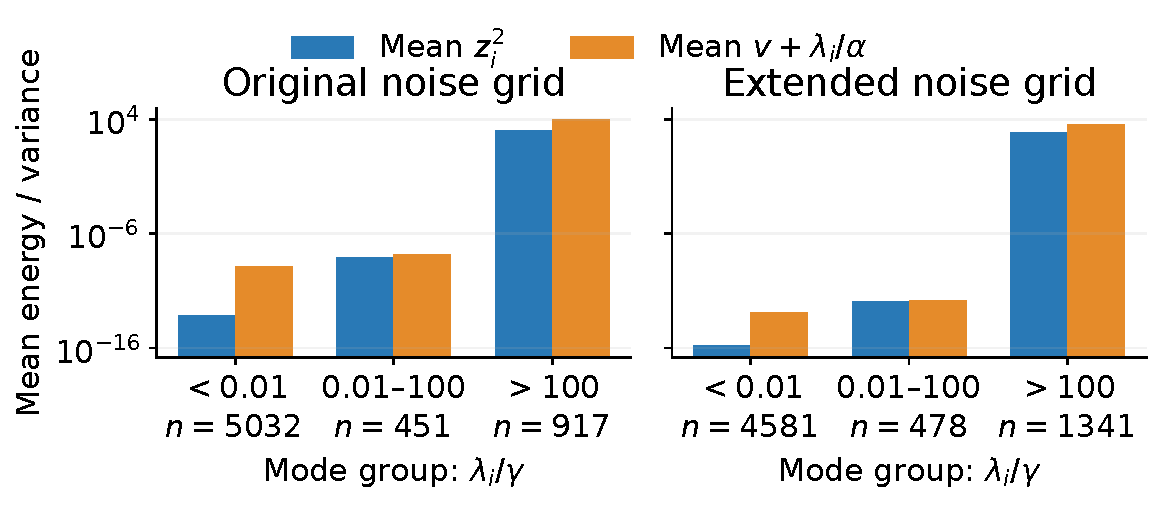
\includegraphics[width=.86\textwidth]{figures/round2_evidence_energy_reference.pdf}
\caption{Burgers--MLP seed $2$, zero-mean prior: projected affine-observation energy $z_i^2$ and model
variance $v+\lambda_i/\alpha$ at the original and extended selections, averaged in three
$\lambda_i/\gamma$ groups. Counts accompany the bars. Little data energy in weak
groups favours lower noise in \eqref{eq:r2-evidence-slope}; the grouping is descriptive.}
\label{fig:r2-evidence-energy}
\end{figure}

\emph{Synthetic validation.}
Dense tests give posterior mean/covariance relative discrepancies at most
$4.90\times10^{-12}$ and $3.01\times10^{-12}$, and log-evidence discrepancy
$1.42\times10^{-13}$. Across $1000$ correctly specified draws, posterior-centred
coverage is $0.6870$ (SE $0.00544$) at one sigma and $0.9534$ (SE $0.00249$) at
$1.96$ sigma. A full-column-rank fit with $N=40,P=12,v=0.2$ gives mean residual-noise
MLE $0.140411$ (SE $0.001198$), consistent with $(N-P)v/N=0.14$ rather than $v$.
In each $100$-draw evidence toy, including a $21.2$-decade spectrum with $79/96$
eigenvalues below $\varepsilon_{64}\lambda_{\max}$, all selected pairs are interior and
agree with the prescribed-spectrum reference. The stressed toy nevertheless fails its
whole-grid $10^{-7}$ scaled tolerance, with maximum discrepancy
$4.55\times10^{-5}$, despite selected log-evidence discrepancies at most
$9.40\times10^{-8}$. Appendix~\ref{oa:numerics} gives scale-estimation distributions and
the failed check; these controls do not establish PINN evidence stability.

\emph{Centre and regional displacement.}\label{app:r2:centres}
Table~\ref{tab:r2-centres} compares the prior centres and nonlinear diagnostic at fixed
baseline/MLE scales; Table~\ref{tab:r2-relative-shift} reports relative regional
displacements. A reduced error contrast need not improve accuracy. Covariance
is shared, whereas errors and coverage are centre-specific.
At the conditional MLE, all eight Burgers--MLP zero-mean-prior affine gaps lie in
$[1.51,3.39]$; one-standard-deviation coverage is $0.9815$--$0.99998$ in bulk
and $0.4185$--$0.92475$ in sharp. The trained-centre allocation reversals and
bulk undercoverage therefore do not transfer to this centre.

% Generated by scripts/make_paper_tables.py from reviewed theta outputs.
\begin{table}[t]
\centering\small\setlength{\tabcolsep}{3pt}
\begin{tabular}{@{}lrr*{6}{r}@{}}
\toprule
 & & & \multicolumn{3}{c}{Baseline} & \multicolumn{3}{c}{Conditional MLE} \\
\cmidrule(lr){4-6}\cmidrule(l){7-9}
family & $n$ & trained & zero & $\theta$ & nonlinear & zero & $\theta$ & nonlinear \\
\midrule
Burgers--MLP & $8$ & $0.02546$ & $0.05883^{(7)}$ & $0.02537^{(2)}$ & $0.02537^{(2)}$ & $0.023^{(5)}$ & $0.02283^{(2)}$ & $0.03944^{(6)}$ \\
Burgers--Fourier & $3$ & $0.05124$ & $0.04316^{(1)}$ & $0.05118^{(0)}$ & $0.05118^{(0)}$ & $0.04235^{(0)}$ & $0.04935^{(0)}$ & $0.05091^{(1)}$ \\
Allen--Cahn--MLP & $3$ & $0.03287$ & $0.2776^{(3)}$ & $0.03275^{(0)}$ & $0.03275^{(0)}$ & $0.02804^{(1)}$ & $0.02455^{(0)}$ & $0.2701^{(3)}$ \\
Allen--Cahn--Fourier & $3$ & $0.03351$ & $0.245^{(3)}$ & $0.03349^{(0)}$ & $0.03349^{(0)}$ & $0.03975^{(1)}$ & $0.02496^{(0)}$ & $0.03861^{(1)}$ \\
\bottomrule
\end{tabular}
\caption{Paired full-grid RMS prediction errors. Entries are unweighted means
of per-run RMS errors; superscripts count runs worse than the trained predictor
out of $n$. Baseline uses $(\alpha_0,1)$ and MLE uses $(\alpha_0,\widehat v)$.
Zero and $\theta$ denote the two affine prior-centre predictions; nonlinear
is $u_{\theta+\delta_L}$, a forward diagnostic rather than a posterior mean.
All comparisons retain the original covariance linearisation.}
\label{tab:r2-centres}
\end{table}


\begin{table}[t]
\centering\small\setlength{\tabcolsep}{4pt}


\begin{tabular}{@{}llrr@{}}
\toprule
family & region & baseline & MLE \\
\midrule
Burgers--MLP & bulk & $[7.54,54.1]$ & $[0.264,1.51]$ \\
 & sharp & $[0.58,57.7]$ & $[0.108,8.55]$ \\
Burgers--Fourier & bulk & $[3.87,8.31]$ & $[0.823,2.42]$ \\
 & sharp & $[0.666,0.864]$ & $[0.167,0.809]$ \\
Allen--Cahn--MLP & bulk & $[15.7,23]$ & $[1.57,2.59]$ \\
 & sharp & $[5.46,7.22]$ & $[0.416,0.628]$ \\
Allen--Cahn--Fourier & bulk & $[8.94,9.95]$ & $[0.97,1.09]$ \\
 & sharp & $[4.38,6.25]$ & $[0.36,2.26]$ \\
\bottomrule
\end{tabular}
\caption{Across-run ranges of total regional RMS zero-mean-prior affine displacement divided by trained
error RMS on the same full-time region. Baseline is $(\alpha_0,1)$ and MLE is
$(\alpha_0,\widehat v)$. Displacement alone does not determine prediction accuracy;
its alignment with trained error matters. Appendix~\ref{oa:empirical} includes transition
regions and evidence settings.}
\label{tab:r2-relative-shift}
\end{table}

\emph{Sampled oracle and post-formation coverage.}
At every saved $\gamma$, centre and subset, a higher empirical bulk-$0.68$ quantile of
$|e_c|/\sigma$ supplies a width multiplier. Selection minimises $|\log\rho|$ across
distinct saved precisions, with lowest $\gamma$ breaking ties. This reference-error
oracle uses sampled settings. Trained Burgers--MLP
seeds $0,4,5,6,7$ have full-time sampled crossing brackets; six zero-mean affine full-time
and six post-formation curves have brackets. Full-time zero-mean affine seeds $1,7$ and
post-formation seeds $1,3$ stay above one at every saved point.

% Derived only from frozen production/review archives; no new grid or checkpoint evaluation.
\begin{table}[t]
\centering\footnotesize\setlength{\tabcolsep}{4pt}


\begin{tabular}{@{}llrrrr@{}}
\toprule
family & subset & trained $68\%$ & affine $68\%$ & trained $95\%$ & affine $95\%$ \\
\midrule
Burgers--MLP & full & $[0.3427,\,0.8605]$ & $[0.164,\,0.9815]$ & $[0.639,\,0.9742]$ & $[0.298,\,0.995]$ \\
Burgers--MLP & post & $[0.1639,\,0.9959]$ & $[0.008972,\,0.3467]$ & $[0.4176,\,1]$ & $[0.01387,\,0.7121]$ \\
Burgers--Fourier & full & $[0.1985,\,0.5978]$ & $[0.2828,\,0.4662]$ & $[0.4472,\,0.7588]$ & $[0.5145,\,0.742]$ \\
Burgers--Fourier & post & $[0.01713,\,0.0938]$ & $[0.08972,\,0.3173]$ & $[0.03589,\,0.1819]$ & $[0.1998,\,0.5571]$ \\
Allen--Cahn--MLP & full & $[0.0095,\,0.0655]$ & $[0.2015,\,0.2755]$ & $[0.0395,\,0.2722]$ & $[0.3588,\,0.3962]$ \\
Allen--Cahn--Fourier & full & $[0.1477,\,0.2005]$ & $[0.0775,\,0.3827]$ & $[0.2407,\,0.4138]$ & $[0.1432,\,0.7338]$ \\
\bottomrule
\end{tabular}
\caption{Across-run sharp-region coverage ranges for trained and zero-mean-prior affine centres at each run's closest saved contrast setting, chosen separately for each centre and subset. A closest sample need not have $\rho\approx1$, so these rows do not generally evaluate coverage after RMS-contrast matching. At each saved $\gamma$, a higher empirical bulk-$0.68$ quantile supplies the width multiplier; selection minimises $|\log\rho|$ and the lowest saved $\gamma$ breaks exact ties. These reference-error oracles use all $8$ Burgers--MLP or $3$ other admitted runs, including runs without a crossing. ``Post'' uses the unchanged global masks intersected with Burgers $t\ge1/\pi$. Bulk one-sigma coverage is about $0.68002$; neither nominal sharp coverage nor an exact root is enforced.}
\label{tab:r2-oracle}
\end{table}


For Burgers, post-formation masks intersect unchanged global masks with
$t\ge1/\pi$, yielding $48{,}246$ bulk, $4928$ transition and $1226$ sharp points.
Table~\ref{tab:r2-oracle} includes all runs, including those without crossings; the
closest sample need not have $\rho\approx1$. Its coverage ranges distinguish regional
contrast from calibration. Saved modal sums refine the five trained-centre crossings;
direct root fields confirm their coverage envelopes (Table~\ref{tab:r3-roots}).
These precisions are not contrast-matching roots for the other centres.
Appendix~\ref{oa:empirical} gives per-run curves.

\emph{Predictive bounds for the prior-centre comparison.}\label{app:r3:centres}
For $\gamma,v>0$, write $A_\gamma=F+\gamma I$. The zero-mean-prior shift splits as
\[
 \delta_\gamma=\delta_{L,\gamma}+\delta_{P,\gamma},\qquad
 \delta_{L,\gamma}=-A_\gamma^{-1}J^\top r,\qquad
 \delta_{P,\gamma}=-\gamma A_\gamma^{-1}\theta.
\]
In the factorisation above, their coordinates are
$-s_i(V^\top r)_i/(s_i^2+\gamma)$ and
$-\gamma\theta_{\rm modes,i}/(s_i^2+\gamma)$; the QR-complement contributions
are $0$ and $-Q_cQ_c^\top\theta$, respectively. The total norm includes their
cross term. Replacing the prior by $\vartheta\sim\mathcal N(\theta,\alpha^{-1}I)$
removes $\delta_{P,\gamma}$ and leaves the covariance unchanged.

Define $\mathcal K_\gamma=r^\top J A_\gamma^{-1}J^\top r$ and
$c_\gamma=\sqrt{\mathcal K_\gamma/v}$. Since
$\delta_{L,\gamma}^\top A_\gamma\delta_{L,\gamma}=\mathcal K_\gamma$,
Cauchy--Schwarz in the $A_\gamma$ metric gives the pointwise bound
\begin{equation}\label{eq:r3:centre-bound}
 |m^\theta_\gamma(x)-u_\theta(x)|
 =|g(x)^\top\delta_{L,\gamma}|
 \le\sigma(x)c_\gamma,\qquad
 \mathcal K_\gamma=\sum_i\frac{s_i^2(V^\top r)_i^2}{s_i^2+\gamma}.
\end{equation}
Let $E_r$ and $\Sigma_r$ denote trained error RMS and uncertainty RMS, and let
$q_{r,i}$ be the regional mode energies in \eqref{eq:r2-regional-modal}.
The regional RMS triangle inequality also gives
\begin{equation}\label{eq:r3:regional-bound}
 B_r=\min\!\left\{c_\gamma\Sigma_r,
              \sum_i|\delta_{L,\gamma,i}|\sqrt{q_{r,i}}\right\},\qquad
 \max(0,E_r-B_r)\le E^\theta_r\le E_r+B_r.
\end{equation}
For $E^\theta_{\mathcal B}>0$ and $\Rrms>0$,
$\rho^\theta\ge\max(0,E_{\mathcal S}-B_{\mathcal S})/
[(E_{\mathcal B}+B_{\mathcal B})\Rrms]$.
The prior-only prediction differs from
the archived zero-mean affine mean by $g^\top\delta_L$; its full-grid error is
therefore at least $E^{\rm zero}_{\rm full}-B_{\rm full}$. This attributes
worsening through a prediction-level bound rather than parameter norms.
If $C_c(t)$ denotes empirical coverage at $t$ standard deviations, then
\[
 C_{\rm trained}(t-c_\gamma)\le C_\theta(t)
       \le C_{\rm trained}(t+c_\gamma),\qquad t\ge c_\gamma,
\]
by the pointwise triangle inequality.

% Derived from round3_local/outputs/summary.json, 12 October 2026.
The saved-array calculation reproduces all $401$ total displacement norms to
$4.44\times10^{-16}$ relative and regional variances to $6.73\times10^{-14}$.
Across those settings, $\|\delta_\gamma\|/\|\theta\|$ ranges from approximately
$0.9889$ to $31.17$; these displacements do not validate a nonlinear first-order approximation.
At the baseline, $\|\delta\|/\|\theta\|$ is $[0.997775,0.999576]$, whereas
$\|\delta_L\|/\|\theta\|$ is $[8.73\times10^{-6},1.5413\times10^{-4}]$;
the QR-complement norm alone is $[0.976675,0.985087]\|\theta\|$.
Using \eqref{eq:r3:centre-bound} and \eqref{eq:r3:regional-bound} gives
$c_\gamma\in[0.007489,0.090775]$ and, after the
regional refinement, establishes a $\theta$-centred allocation deficit in $16/17$
runs from bounds alone. Its seed-$4$ lower bound $0.4878$ is inconclusive;
direct predictions establish the deficit in all $17$ (Section~\ref{sec:ceiling}).
The prior-only prediction is worse in all $14$ baseline cases where the
zero-mean affine prediction worsens.
The $\theta$-centred one-sigma coverage lower bounds are $0.7925$ in sharp and
$0.997196$ in bulk, so both regions overcover in all $17$ runs. Bulk $1.96$-sigma
coverage is $1$; sharp $1.96$-sigma coverage is above nominal in $12$ runs and
below nominal in the other $5$. Their upper bounds are $0.924$, $0.883$,
$0.90875$, $0.91225$ and $0.896$ for Burgers--MLP seeds $1,2,3$ and
Burgers--Fourier seeds $0,6$, respectively. At the conditional MLE,
$c_\gamma\in[75.428,79.910]$ is uninformative; Table~\ref{tab:r2-centres} instead
reports the directly evaluated alternative centre.


\emph{Coverage envelopes at refined contrast-matching roots.}\label{app:r3:root-envelope}
At unit noise, each pointwise variance has the positive modal representation
$q_\gamma(x)=\sum_i a_i(x)/(\lambda_i+\gamma)$, including the QR complement
as a zero-eigenvalue mode, with $a_i(x),\lambda_i\ge0$.
For positive endpoint variances at saved precisions
$0<l\le\gamma\le h$, $l<h$, and
$t=(\gamma-l)/(h-l)$, positivity gives
\begin{equation}\label{eq:r3:variance-envelope}
 L_\gamma=\frac{(1-t)lq_l+thq_h}{\gamma}
 \le q_\gamma\le
 U_\gamma=\left(\frac{1-t}{q_l}+\frac{t}{q_h}\right)^{-1}.
\end{equation}
For the lower bound in \eqref{eq:r3:variance-envelope}, $\gamma q_\gamma$ is concave because every
$\gamma/(\lambda_i+\gamma)$ is concave. For the upper bound,
$q'=-\sum_i a_i/(\lambda_i+\gamma)^2$ and
$q''=2\sum_i a_i/(\lambda_i+\gamma)^3$ satisfy
$(q')^2\le qq''/2$ by Cauchy--Schwarz. Hence
$(1/q)''=[2(q')^2-qq'']/q^3\le0$, and taking the reciprocal of its chord gives
$U_\gamma$. Both envelopes decrease with $\gamma$ since $q_l\ge q_h$.

For a numerically refined root bracket $[a,b]\subset[l,h]$, use $L_b$ and
$U_a$ to retain root-location uncertainty. The higher empirical bulk-$0.68$
quantile $Q_{\mathcal B}$ is monotone, so
\[
 k_{\min}=Q_{\mathcal B}(|e|/\sqrt{U_a}),\qquad
 k_{\max}=Q_{\mathcal B}(|e|/\sqrt{L_b})
\]
enclose the multiplier $k_\gamma$ that calibrates bulk coverage at the root.
For sharp coverage at threshold $z\ge0$, this yields
\begin{equation}\label{eq:r3:coverage-envelope}
 \left\langle\mathbf1\{|e|\le z k_{\min}\sqrt{L_b}\}\right\rangle_{\mathcal S}
 \le C_{\mathcal S,\gamma}(z)\le
 \left\langle\mathbf1\{|e|\le z k_{\max}\sqrt{U_a}\}\right\rangle_{\mathcal S}.
\end{equation}
These analytic bounds use the returned spectral model and saved endpoint fields;
they are not directed-rounding certificates for the original Jacobian.
Direct pointwise root evaluations confirm the enclosures in Table~\ref{tab:r3-roots}.
Root refinement concerns the five observed
trained-centre brackets, without asserting uniqueness or global optimality.
Appendix~\ref{oa:lean} maps the Lean verification of these analytic bounds.
The evaluated run counts and refined brackets remain numerical results.

% Generated by scripts/make_paper_tables.py; old bounds and new direct evaluations.
\begin{table}[t]
\centering\small\setlength{\tabcolsep}{4pt}
\begin{tabular}{@{}rrrcr c@{}}
\toprule
 & & \multicolumn{2}{c}{Sharp $1\sigma$ coverage} & \multicolumn{2}{c}{Sharp $1.96\sigma$ coverage} \\
\cmidrule(lr){3-4}\cmidrule(l){5-6}
seed & refined $\gamma$ & direct & envelope & direct & envelope \\
\midrule
$0$ & $0.02105515$ & $0.3275$ & $[0.323,0.333]$ & $0.78275$ & $[0.7815,0.78475]$ \\
$4$ & $0.73626974$ & $0.427$ & $[0.41975,0.43375]$ & $0.852$ & $[0.84525,0.862]$ \\
$5$ & $2.0476385\times10^{-5}$ & $0.30325$ & $[0.29775,0.315]$ & $0.67725$ & $[0.6755,0.67925]$ \\
$6$ & $0.00163541$ & $0.52325$ & $[0.5225,0.526]$ & $0.847$ & $[0.8465,0.84775]$ \\
$7$ & $3.0590419\times10^{-5}$ & $0.55725$ & $[0.554,0.563]$ & $0.8235$ & $[0.82125,0.82675]$ \\
\bottomrule
\end{tabular}
\caption{Direct sharp coverage and saved envelopes at five trained Burgers--MLP
roots. Displayed precisions are rounded; root brackets have relative width below
$5.3\times10^{-13}$. Bulk calibration uses the higher empirical $0.68$ quantile.
Envelopes include root and calibration uncertainty through
\eqref{eq:r3:coverage-envelope}; all direct values lie inside.}
\label{tab:r3-roots}
\end{table}



\emph{Regional calibration and sampled agreement band.}\label{app:r4-oracles}
At each trained-centre closest saved setting, use either
$k_{\mathcal B}=Q_{\mathcal B}(|e|/\sigma;0.68)$ or
$k_{\mathcal S}=Q_{\mathcal S}(|e|/\sigma;0.68)$, with the higher empirical quantile.
Write $C^r_{\mathcal S}(z)=\langle\mathbf1\{|e|\le z k_r\sigma\}\rangle_{\mathcal S}$
and $Z^r=e/(k_r\sigma)$ for the resulting coverage and standardised errors.
Table~\ref{tab:r4-oracles} gives full-grid per-seed results and family ranges,
including the Burgers post-formation subsets. Sharp calibration fixes its
one-standard-deviation coverage by construction: $0.68025$ on $4000$ full-grid
sharp points and $0.68108$ on $1226$ post-formation points here. The informative
outputs are coverage at $1.96$ standard deviations and the absolute and signed
standardised means. These are finite-grid descriptions, not repeated-draw guarantees.
Inclusive quantile comparisons can differ by one point from older multiplied-width
arithmetic; all continuous summaries reproduce to relative tolerance $10^{-12}$.

The band inventory retains every distinct saved precision with $0.9\le\rho\le1.1$:
$28$ run/subset settings across the full grids and Burgers post-formation masks.
For Burgers--MLP seed $7$, the seven full-grid samples give sharp coverage
$0.44725$--$0.986$ at one standard deviation and $0.78375$--$1$ at $1.96$ after
bulk calibration. Their $\rho$ values span $0.90635$--$1.06370$; nearby contrast
values need not correspond to nearby precisions on a nonmonotone curve.
The other four crossing seeds each have one saved full-grid point in the band,
with one-standard-deviation coverages $0.34275$, $0.437$, $0.35925$ and $0.5165$
for seeds $0,4,5,6$. The archived per-run inventory is sampled rather than a
continuous-band enclosure; Table~\ref{tab:r3-roots} retains the separate refined-root bounds.

% Recomputed from frozen round-two fields by analysis/round4_local/review_round4.py.
\begin{table}[!tb]
\centering\small\setlength{\tabcolsep}{4pt}
\begin{tabular}{@{}lrrrrrr@{}}
\toprule
Burgers--MLP seed & $\rho$ & $C^{\mathcal B}_{\mathcal S}(1)$ & $C^{\mathcal B}_{\mathcal S}(1.96)$ & $C^{\mathcal S}_{\mathcal S}(1.96)$ & $\overline{|Z|}^{\mathcal S}$ & $\overline Z^{\mathcal S}$\\
\midrule
0 & 0.95438 & 0.34275 & 0.7885 & 0.92025 & 0.91339 & $-0.24502$ \\
1 & 1.8363 & 0.8605 & 0.97425 & 0.865 & 0.94283 & $0.85765$ \\
2 & 2.5874 & 0.44675 & 0.639 & 0.85025 & 1.3644 & $1.209$ \\
3 & 1.9924 & 0.725 & 0.933 & 0.9175 & 0.77179 & $0.56348$ \\
4 & 0.95486 & 0.437 & 0.86375 & 0.95775 & 0.83109 & $-0.069397$ \\
5 & 0.97331 & 0.35925 & 0.69175 & 0.8345 & 1.0436 & $-1.0371$ \\
6 & 1.0323 & 0.5165 & 0.8435 & 0.92825 & 0.85021 & $0.069544$ \\
7 & 0.96422 & 0.65175 & 0.837 & 0.84675 & 1.034 & $0.79421$ \\
\midrule
\multicolumn{2}{l}{Family / subset ($n$)} & \multicolumn{2}{c}{$C^{\mathcal S}_{\mathcal S}(1.96)$} & $\overline{|Z|}^{\mathcal S}$ & \multicolumn{2}{c}{$\overline Z^{\mathcal S}$}\\
\midrule
\multicolumn{2}{l}{Burgers--MLP / full ($8$)} & \multicolumn{2}{c}{$[0.8345,\,0.95775]$} & $[0.77179,\,1.3644]$ & \multicolumn{2}{c}{$[-1.0371,\,1.209]$} \\
\multicolumn{2}{l}{Burgers--Fourier / full ($3$)} & \multicolumn{2}{c}{$[0.82475,\,0.85075]$} & $[1.0792,\,1.3448]$ & \multicolumn{2}{c}{$[0.98518,\,1.3234]$} \\
\multicolumn{2}{l}{Allen--Cahn--MLP / full ($3$)} & \multicolumn{2}{c}{$[0.921,\,0.959]$} & $[0.77708,\,0.86039]$ & \multicolumn{2}{c}{$[-0.29925,\,0.32371]$} \\
\multicolumn{2}{l}{Allen--Cahn--Fourier / full ($3$)} & \multicolumn{2}{c}{$[0.98325,\,0.9995]$} & $[0.71247,\,0.81491]$ & \multicolumn{2}{c}{$[-0.36263,\,0.27285]$} \\
\multicolumn{2}{l}{Burgers--MLP / post ($8$)} & \multicolumn{2}{c}{$[0.94454,\,1]$} & $[0.61868,\,0.98575]$ & \multicolumn{2}{c}{$[-0.87154,\,0.82267]$} \\
\multicolumn{2}{l}{Burgers--Fourier / post ($3$)} & \multicolumn{2}{c}{$[0.8646,\,1]$} & $[0.82852,\,0.87527]$ & \multicolumn{2}{c}{$[0.7548,\,0.86578]$} \\
\bottomrule
\end{tabular}
\caption{Trained-centre regional calibration at each run's closest saved contrast setting.
The superscript $\mathcal B$ or $\mathcal S$ denotes the region whose higher empirical
$0.68$ quantile supplies the width multiplier. The upper panel gives eight full-grid
Burgers--MLP seeds; the lower panel gives observed ranges for all $17$ full-grid runs
and the Burgers post-formation subsets. Each setting minimises $|\log\rho|$, with ties
at the lowest saved precision. $\overline{|Z|}^{\mathcal S}$ and $\overline Z^{\mathcal S}$
are absolute and signed means of sharp-calibrated standardised errors.
Sharp one-standard-deviation coverage is fixed by construction, up to discreteness
and ties. Displayed values are rounded; reference calibration does not define a training rule.}
\label{tab:r4-oracles}
\end{table}


\emph{Width versus allocation.}
At $v=1$, changing $\gamma$ changes modal weights. At fixed $\gamma=\alpha_0$,
varying $v$ with $\alpha=\alpha_0/v$ multiplies widths by $\sqrt v$ without changing
contrast: $\meanZ$ scales as $v^{-1/2}$ and coverage is the empirical CDF of fixed
standardised errors at $\sqrt v$. Figure~\ref{fig:r2-coverage-scale} shows both effects;
the fixed-$\gamma$ curves are rescalings of saved fields, not fitted scales.

\begin{figure}[!t]
\centering
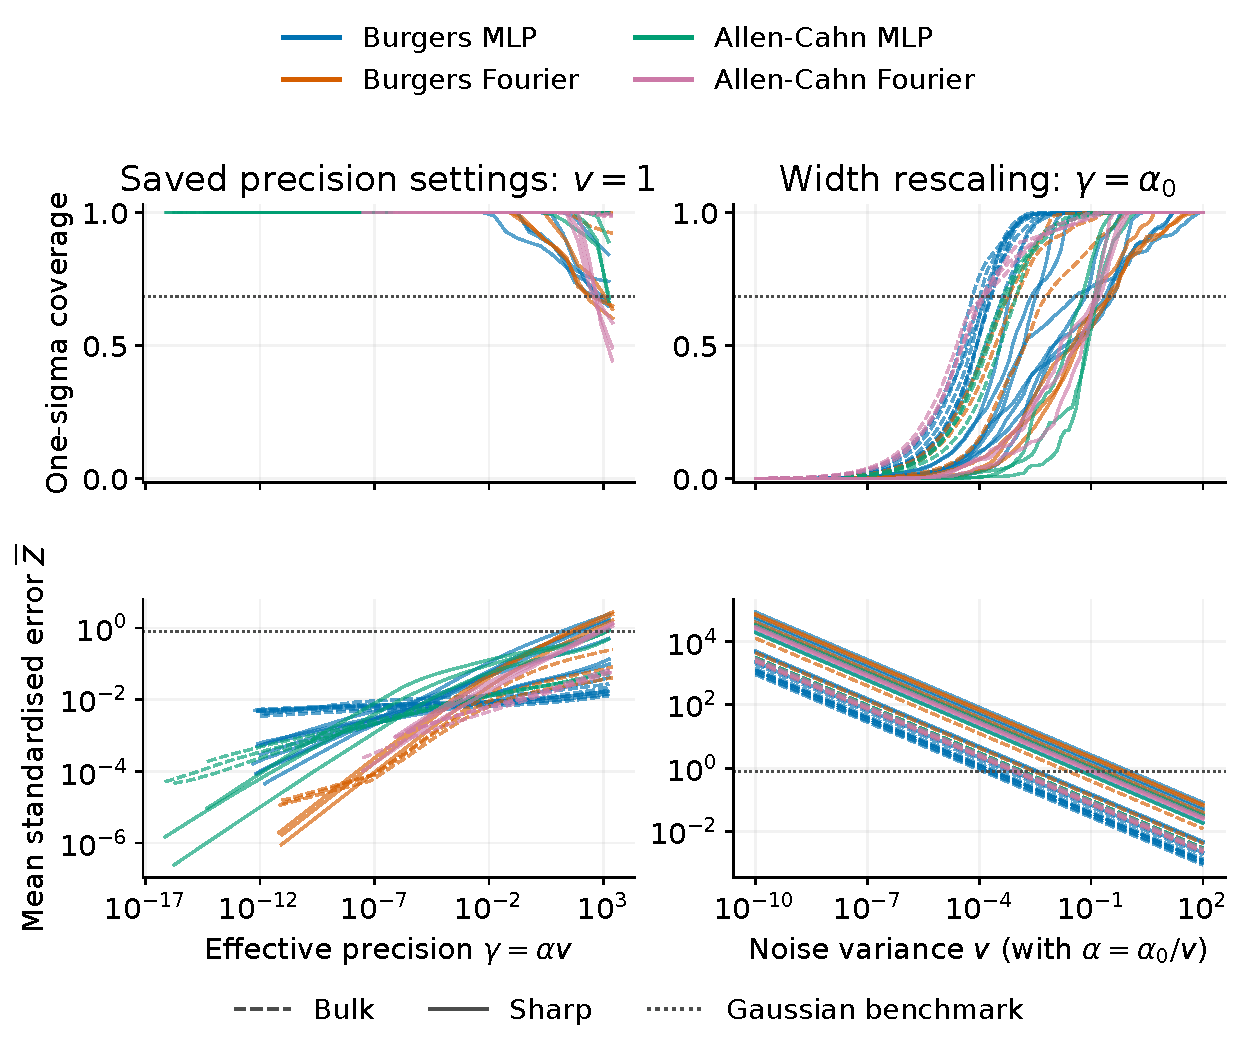
\includegraphics[width=.95\textwidth]{figures/round2_coverage_scale.pdf}
\caption{Trained-centre one-sigma coverage and mean standardised error for all $17$
full-time runs. Colours identify families; dashed/solid curves denote bulk/sharp.
Left: saved precisions at $v=1$; right: width rescaling at $\gamma=\alpha_0$.
Dotted lines mark Gaussian expectations $0.68269$ and $0.79788$.
Lines join evaluated points without asserting confidence intervals.}
\label{fig:r2-coverage-scale}
\end{figure}


